% !TEX root = ../thesis.tex
After seeing where the Lattice Boltzmann Method originated, we now take a closer look at how the method is derived.

As of today, the most intuitive way of deriving the \gls{lbm} is to start at the Boltzmann equation.
It describes the evolution of the so-called \textbf{\gls{pdf}}\footnote{Important new vocabulary and vectorial quantities will be highlighted in bold font for easier recognition} $f(\vec{v},\vec{x},t)$, which gives the probability of finding a particle at spacial position $\vec{x}$ and time $t$ with microscopic velocity $\vec{v}$:
\begin{equation}
  \label{eq: Boltzmann transport equation}
  \frac{\partial f}{\partial t} (\vec{v},\vec{x},t) + \vec{v} \cdot \nabla_{\vec{x}} f(\vec{v},\vec{x},t) = \Omega\left(f(\vec{v},\vec{x},t)\right),
\end{equation}
where $\Omega$ describes the effect of the collision of two particles. The other part is just the total time derivative\footnote{leaving out external forces} $\frac{\text{d}f}{\text{d}t}$.
To see the difficulty of the Boltzmann equation, we need to write out the collision $\Omega$:
\begin{equation}
  \label{eq: Collision of boltzmann equation}
  \begin{aligned}
 \Omega\left(f(\vec{v},\vec{x},t)\right) =\frac{1}{m}
  \int \left( \vec{\tilde{v}_1}-\vec{\tilde{v}_2}\right)
  \left[
    f(\vec{\tilde{v}_1},\vec{x},t)f(\vec{\tilde{v}_2},\vec{x},t)
    -f(\vec{v},\vec{x},t)f(\vec{v_2},\vec{x},t)
  \right] d\phi d\vec{v_2}
\end{aligned}
\end{equation}
The right hand side is the aforementioned integral term which includes the mass $m$ of the particles and the post-collision velocities $\vec{\tilde{v}_1}$ and $\vec{\tilde{v}_2}$.
Those velocities are dependent on the collision angle $\phi$ and the pre-collision velocities $\vec{v}$ and $\vec{v_2}$ and have to be integrated over all possible collision scenarios.
More background information on this equation can be found in~\cite{harris2004introduction}.

Additionally, by the definition of an \textbf{equilibrium}, the \glspl{pdf} $f^{eq}$ in an equilibrium have to fulfill $\frac{\text{d}f^{eq}}{\text{d}t}=0$ and hence
\begin{equation}
  \Omega(f^{eq}(\vec{v},\vec{x},t)) = 0,
\end{equation}
i.e.\ the collision of the particles has no effect on their distribution function.
Those distributions are called equilibrium distributions and are unique for a given velocity.
In the rest of this thesis, values derived from the equilibrium distributions will be denoted by a superscript $eq$.

The silver lining in this setting is, that we can extract multiple equations for fluid dynamics from~\eqref{eq: Boltzmann transport equation}, without the need to calculate the right hand side~\eqref{eq: Collision of boltzmann equation} explicitly.
Using only certain properties of $\Omega$, c.f.~\cite[Pages 26 ff.]{harris2004introduction}, we can for example derive the Navier-Stokes equations.
In this sense, the Boltzmann equation is a more general view of gas dynamics than Navier-Stokes.
\begin{figure}
\centering
% !TEX root = ../../thesis.tex
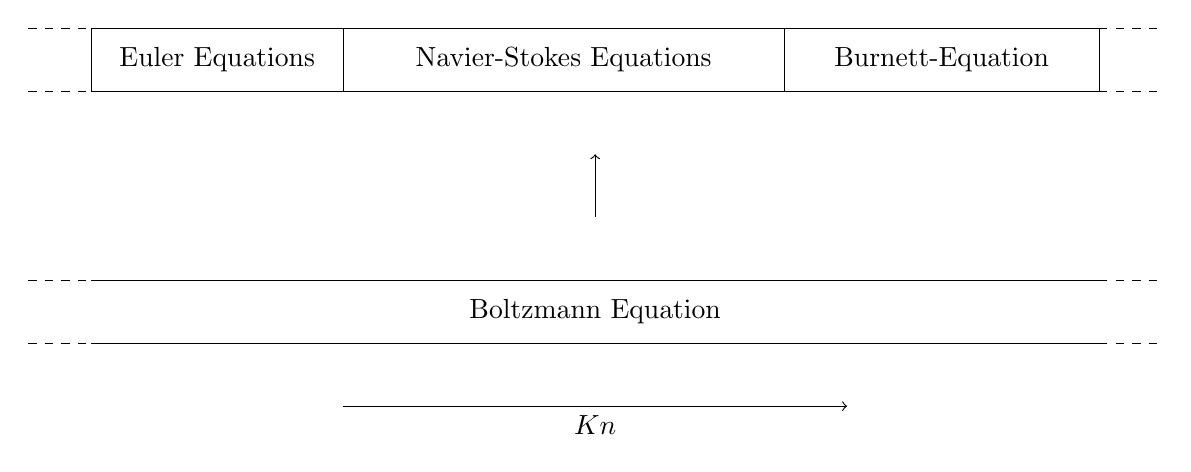
\begin{tikzpicture}[ scale=.8]
\draw[style=dashed] (0,0) -- (1, 0);
\draw[style=dashed] (0,1) -- (1, 1);
\draw (1,0) rectangle (5,1) node[pos=.5] {Euler Equations};
\draw (5,0) rectangle (12,1) node[pos=.5] {Navier-Stokes Equations};
\draw (12,0) rectangle (17,1) node[pos=.5] {Burnett-Equation};
\draw[style=dashed] (17,0) -- (18, 0);
\draw[style=dashed] (17,1) -- (18, 1);

\draw[->] (9,-2) -- (9,-1);

\draw[draw=white] (1,-3) rectangle (17,-4) node[pos=0.5] {Boltzmann Equation};
\draw[style=dashed] (0,-3) -- (1, -3);
\draw[style=dashed] (17,-3) -- (18, -3);
\draw (1,-3) -- (17, -3);
\draw[style=dashed] (0,-4) -- (1, -4);
\draw[style=dashed] (17,-4) -- (18, -4);
\draw (1,-4) -- (17, -4);

\draw[->] (5,-5) -- (13, -5) node[midway, below] {$Kn$};

\end{tikzpicture}

\caption{Range of Boltzmann Equation versus classical equations of fluid dynamics, where $Kn$ is defined in~\eqref{eq: definition of knudsen number}.}
\label{fig: boltzmann vs navier stokes}
\end{figure}

This is one of the advantages of using the Boltzmann equation over Navier-Stokes, summarized in Figure~\ref{fig: boltzmann vs navier stokes}.

To be more precise, one needs the so called continuum hypothesis to use the Navier-Stokes equations, stating roughly that there have to be enough fluid particles in any given control volume for averaging processes to make sense.
Only this hypothesis justifies the notations of density, pressure and temperature, being macroscopic, averaged values of a fluid.
One can concretize this definition by introducing the \gls{kn}, named after the Dutch physicist Martin Knudsen.
It relates the mean free path $\lambda$ a particle can travel before colliding with another particle to the physical scale of the problem represented by a characteristic length $L$ of the problem like
\begin{equation}
  \label{eq: definition of knudsen number}
  Kn=\frac{\lambda}{L}.
\end{equation}
When the Knudsen number is very low, i.e.\ several orders of magnitude below one, we can safely assume the continuum hypothesis.
If either $\lambda$ gets very big, like in high altitudes where the atmosphere is very dilute, or $L$ gets very small like in the simulation of microchannels, $Kn$ is about the order of one and the hypothesis does not hold anymore.
As teased in Figure~\ref{fig: boltzmann vs navier stokes}, there are other equations like the Burnett or Super-Burnett equations, which can handle these regimes.
Nevertheless, they have their very own problems, like being inherently unstable.
The standard reference on this topic is~\cite{agarwal2001beyond}.
